\documentclass[12pt, a4paper]{article}

\usepackage[slovak]{babel}
\usepackage[utf8]{inputenc}
\usepackage[T1]{fontenc}
\usepackage{geometry}
\usepackage{hyperref}
\usepackage{setspace}
\usepackage{subcaption}
\usepackage{afterpage}
\usepackage{graphicx}
\usepackage{csquotes}
\usepackage{longtable}
\usepackage{placeins}
\usepackage{pdfpages}
\usepackage{expl3}

% Dots in TOC
\usepackage{tocloft}
\renewcommand{\cftsecleader}{\cftdotfill{\cftdotsep}}


\setstretch{1.5}
\widowpenalty10000
\clubpenalty10000
\newsavebox\shield
\usepackage{titlesec}

\usepackage[style=iso-numeric,backend=biber]{biblatex}
\addbibresource{literature.bib}
%\AtBeginBibliography{\small}

\geometry{
	a4paper,
	top=2cm,
	left=3cm,
	right=2.5cm,
	bottom=2.5cm
}

\begin{document}
\begin{titlepage}
{\centering
    {\Large Slovenská technická univerzita v Bratislave}\par
    {\Large Fakulta informatiky a informačných technológií}\par
    \vspace{\medskipamount}
    \vfill
    \LARGE \textbf{Inteligentné osvetlenie pracovného stola} \\
    \vspace{0.7\bigskipamount}
    {\Large Semestrálny projekt}\par
    \vfill
}
\normalsize    
\begin{flushleft}
\textbf{Autor:} Bc. Miroslav Hájek \\
\textbf{Študijný program:} Inteligentné softvérové systémy \\
\textbf{Predmet:} Vnorené systémy \\
\textbf{Akademický rok:} 2022 / 2023 \\
\end{flushleft}
\end{titlepage}

\thispagestyle{empty}
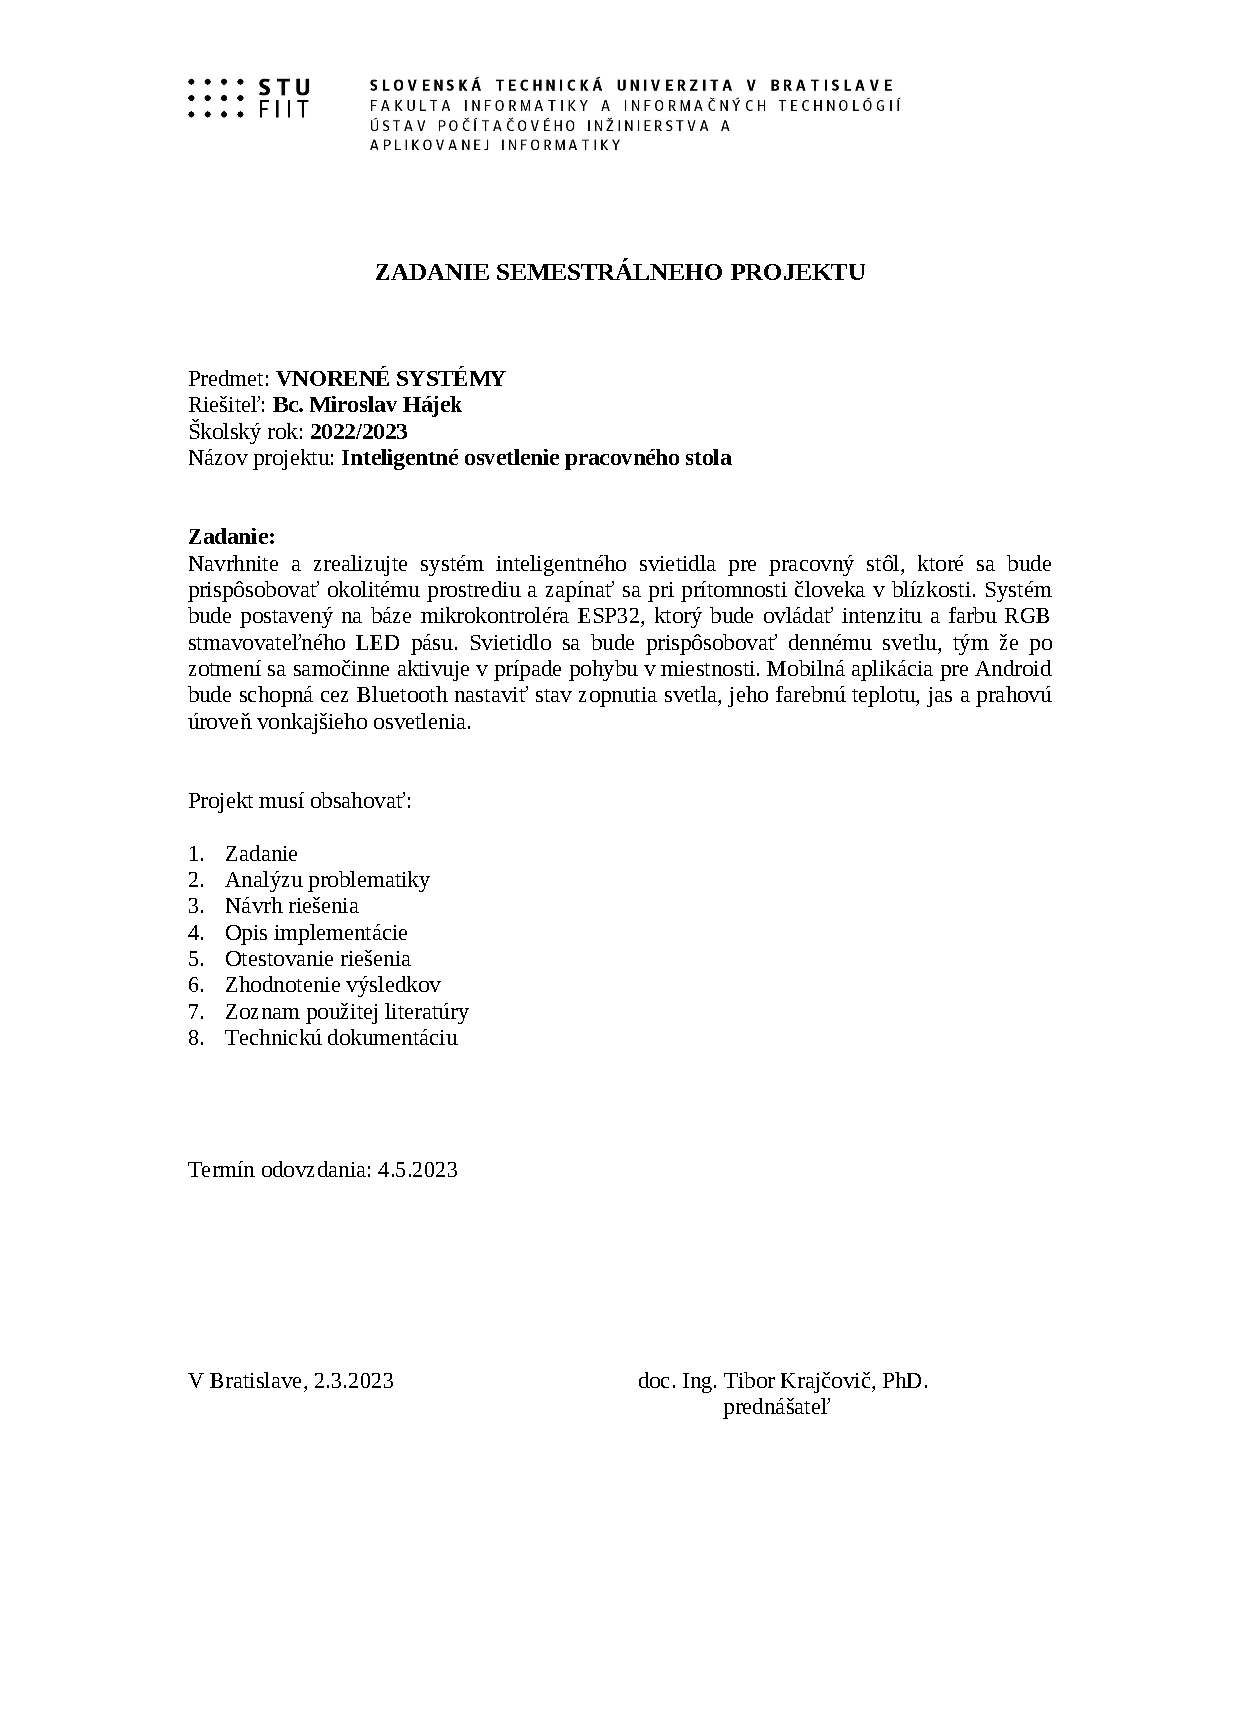
\includepdf[pages=-, scale=1]{zadanie}

\pagenumbering{gobble}
\tableofcontents
\newpage

\pagenumbering{arabic}
\setcounter{page}{1}

\section{Analýza problematiky}
Zariadenie na ovládanie svietidla sa má skladať z dvoch nezávislých integrovaných častí: riadiaca jednotka s firmvérom priamo regulujúca spínanie lampy podľa senzorov, a mobilná aplikácia na zmenu aktívnych nastavení svetla a detekcie pohybu komunikujúca cez Bluetooth. V sekcii popíšeme výber vhodných súčiastok a základné princíp fungovania.

\subsection{Riadiaca jednotka}
Mikrokontrolér \textbf{ESP32 WeMos Lolin D32} (Obr.~\ref{fig:esp32}) sme zvolili spomedzi ostatných bežne dostupných vývojových dosiek (ako sú Arduino, Raspeberry Pi, STM32, BeagleBone a pod.) hlavne pre podporu pre viacerých štandardných mikroprocesorových rozhraní na rozličných pinoch. Doska je postavená na module \emph{ESP32-WROOM-32} \cite{noauthor_esp32-wroom-32_2023}, ktorý disponuje procesorom s frekvenciou 80 MHz (až do 240 MHz) a pamäťou 4 MB Flash a 520 kB SRAM prilíš nelimitujúce rozhodnutia na účely prototypu. 

Napájacie napätie dosky je 3,3 V, ale cez USB konektor môžeme pripojiť zdroj 5 V. ESP-32 sa vyznačuje aj dobrou podporou od výrobcu v podobe SDK obsahujúce ovládače na všetky dostupné rozhrania pre periférie ESP-IDF \cite{noauthor_esp-idf_nodate}, ktorý tiež zahŕňa operačný systém reálneho času FreeRTOS.

\begin{figure}[h]
	\centering
	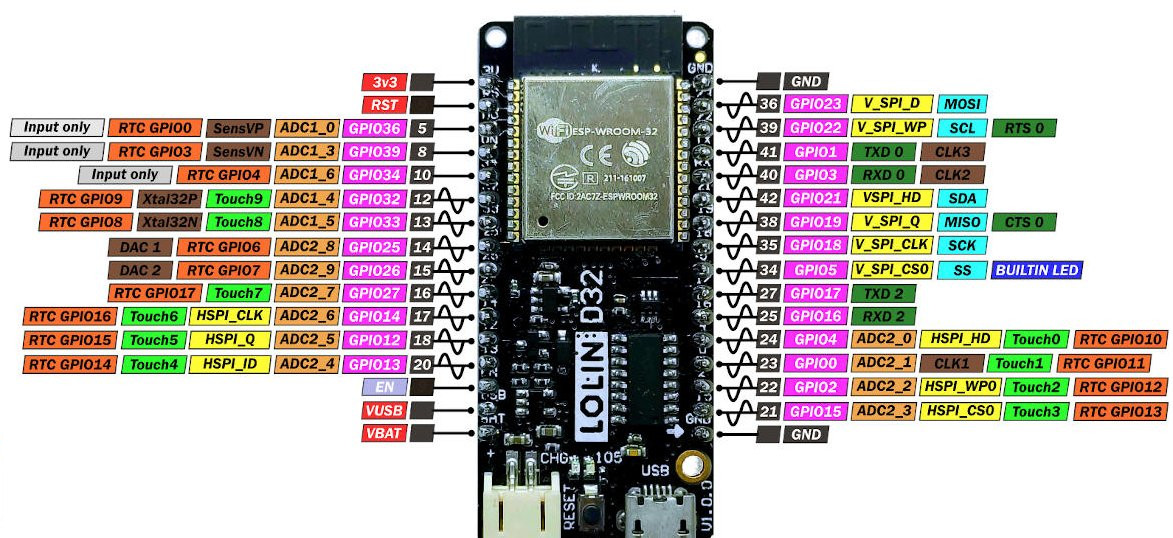
\includegraphics[width=\textwidth]{assets/esp32.jpg}
	\caption{Vývojová doska ESP32 WeMos Lolin D32 \cite{mischianti_esp32_2023}}
	\label{fig:esp32}
\end{figure}

ESP-32 síce disponuje konektivitou na WiFi a Bluetooth, ale funkcie pre RFCOMM nie sú zatiaľ implementované, preto sa Bluetooth komunikácia musí realizovať externým \textbf{modulom HC-05} (Obr.~\ref{fig:hc-05}). Posielanie a príjem správ sa uskutočnuje cez \emph{UART} protokol, kde piny RXD a TXD musia byť na napäťových úroviach 3,3 V, zatiaľ čo napájanie je v rozmedzí 3,6 - 6 V (zväčša 5 V). Baudová rýchlosť je predvolene určená na 9600. 

Pin Enable slúži na prepnutie modulu do AT príkazového režimu (high úroveň), v ktorom je možné upraviť napr. baud. Pin State signalizuje stav Bluetooth pripojenia a je zároveň zapojený na indikačnú LED, ktorá sa môže nachádzať v 3 stavoch: (i) bliknutie raz za 2 sekundy - príkazový režim, (ii) bliknutie 2-krát za 1 sekundu - pripojenie nadviazané, (iii) opakované blikanie - čakanie na pripojenie \cite{noauthor_hc-05_nodate}.

\begin{figure}[h]
	\centering
	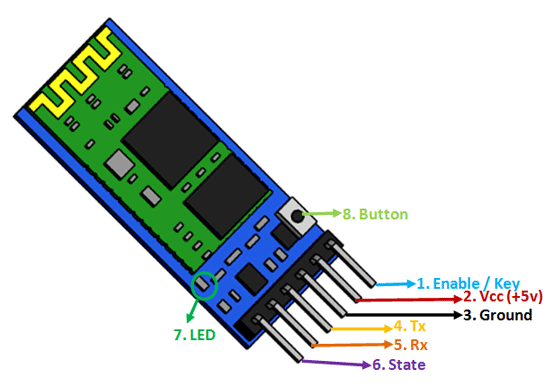
\includegraphics[width=0.5\textwidth]{assets/hc-05.png}
	\caption{Bluetooth modul HC-05 \cite{noauthor_hc-05_nodate}}
	\label{fig:hc-05}
\end{figure}

\subsection{Senzory a akčné členy}
Regulovateľné LED diódy v úlohe akčného členu musia reagovať na situáciu v okolitom prostredí, menovite detekciu pohybu človeka v miestnosti (cez infračervené čidlo) a intenzitu vonkajšieho osvetlenia (cez fotodiódu). 

\subsubsection{RGB LED pásik}
Typ LED pásiku sa vyberá podľa rôznych kritérii ako sú účel použitia, či ide o dekoráciu alebo má slúžiť na osvetlenie miestnosti. Na základe toho prispôsobíme svetelný výkon, farbu, vodovzornosť (stupeň ochrany krytom), rozmery, z čoho nakoniec vyplýva cieľové napätie najčastejšie 12~V, 24~V, 230~V. 

Rozlišujeme pásiky podľa technológie produkcie teplotného odtieňu: jednofarebné, CCT - s dvoma typmi diód 2700~K a 6500~K a reguláciou medzi nimi, RGB - s štvorpinové LED diódami. Svietivosť pásiku ovplyvňuje príkon udávaný na meter, na nasvietenie napr. kuchynskej linky sa odporúča LED pásik s vyšším príkonom 12 - 20 W/m, tie je žiaduce namontovať na hliníkový podklad, z dôvodu chladenia. Ďalší faktor určujúci charakter svetla je rozloženie diód a ich počet na meter pásika \cite{123ledsk_ako_nodate}.

\begin{figure}[h]
\centering
\begin{subfigure}[b]{0.45\textwidth}
	\centering
	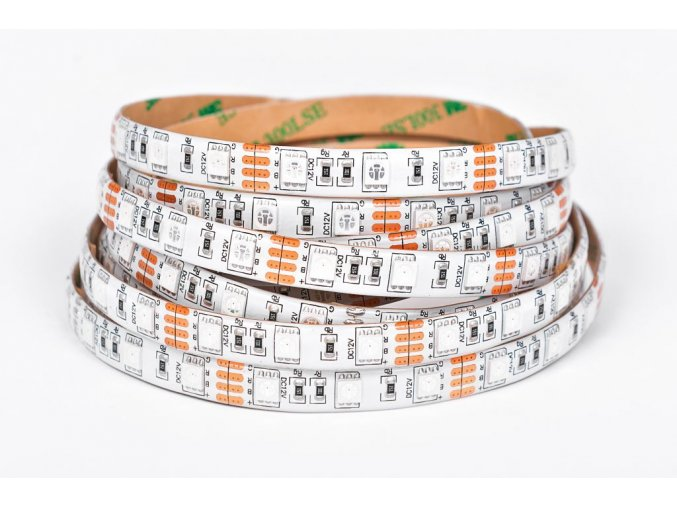
\includegraphics[width=\textwidth]{assets/rgb-led.jpg}
	\caption{LED pásik}
	\label{fig:rgb-led}
\end{subfigure}
\hfill
\begin{subfigure}[b]{0.5\textwidth}
	\centering
	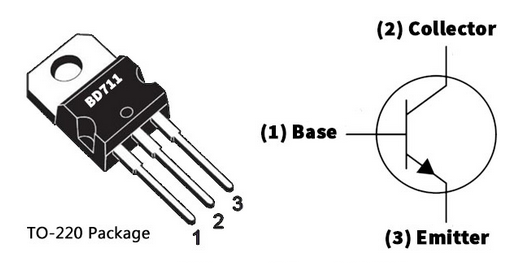
\includegraphics[width=\textwidth]{assets/bd711.png}
	\caption{NPN tranzistor BD711}
	\label{fig:bd-711}
\end{subfigure}
\caption{Akčné členy svietidla}
\end{figure}

Vhodný kandidát na interiérové osvetlenie stola sa ukazuje \textbf{RGB LED pásik} (Obr.~\ref{fig:rgb-led}) so samolepiacou fóliou 3M 300LSE bez krytia IP20, napätím zdroja 12~V, príkonom 14,4~W/m a hustotou diód 60~ks/m, ktorý vyprodukuje až 550~lm/m svetla \cite{123ledsk_rgb_nodate}. LED diódy na pásiku sú zapojenie tri do série so spoločnou anódou v 10 cm oddeliteľných úsekoch. Vetva pre červenú farbu má navyše zapojený do série 300~$\Omega$ SMD rezistor, ostatné vetvy 150~$\Omega$ rezistor.

Jednotlivé farebných kanálov nemôžeme spínať a regulať priamo s pinu mikroprocesoru, pretože nie je prítomné rovnaké napätie: 3,3~V voči 12~V, a nepostačuje ani maximálny prúd $I_{OL}$ = 28 mA. Dedikovaný tranzistor bude spínať prúd do 1,2 A ($I = 14,4W / 12V$), preto potrebujeme výkonovejšie tranzistory ako bežne používaný rad BC ($I_C < 100 mA$). \textbf{NPN tranzistor BD711} (Obr.~\ref{fig:bd-711}) dokáže spínať prúd až do 12 A \cite{noauthor_bd711_nodate}.

\begin{figure}[h]
\centering
\begin{subfigure}[b]{0.4\textwidth}
	\centering
	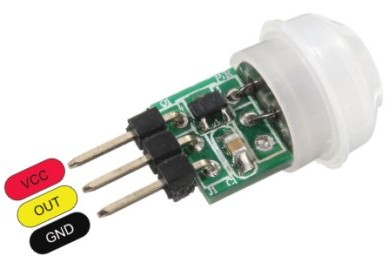
\includegraphics[width=\textwidth]{assets/pir-sb312.jpg}
	\caption{PIR senzor pohybu SB312}
	\label{fig:pir}
\end{subfigure}
\hfill
\begin{subfigure}[b]{0.4\textwidth}
	\centering
	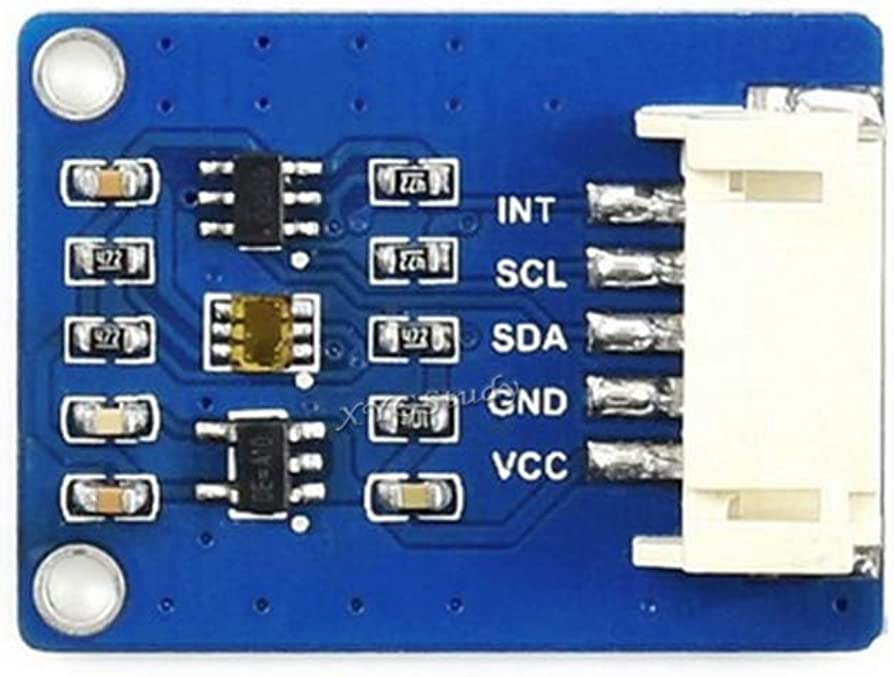
\includegraphics[width=\textwidth]{assets/tsl25911.jpg}
	\caption{Senzor osvetlenia TSL25911}
	\label{fig:light-sensor}
\end{subfigure}
\caption{Senzory s označením vývodov}
\end{figure}

\subsubsection{PIR pohybový senzor}
Na detekciu pohybu ľudí sa používajú infračervené PIR senzory líšiace sa veľkosťou, citlivosťou a nastaviteľnosťou úrovne detektora. Zlepšenie snímacích vlastností je docielené plastovou Fresnelovou šošovkou na senzore. \textbf{Olimex SB312} (Obr.~\ref{fig:pir})sa vyzančuje kompaktnosťou s rozmermi PCB: 10 x 8 mm. Disponuje uhlom snímacieho kužela do 100° s dosahom 3 - 5 metrov. Oneskorenie výstupu voči detegovanému pohybu je 2 sekundy a po rovank dlhý čas podrží výstupnú logickú úroveň v jednotke. Napájacie napätie senzora je 3,3~V \cite{olimex_pir-sb312_nodate}.

\subsubsection{Senzor okolitého osvetlenia}
Modul senzora osvetlenia Waveshare WS-17146 (Obr.~\ref{fig:light-sensor}) obsahuje obvod TSL25911FN, ktorý samostatne prerátava nameranú intenzitu svetla na fotodióde do luxov s použím vzorca na aproximáciu ľudského videnia. Senzor pracuje na napätí 3,3~V aj 5~V a komunikuje cez I2C zbernicu do 400 kbit/s na adrese 0x29. Najdôležitejšie registre pre odčítanie aktuálnej hodnoty sú Control (0x01) a ALS Data (0x14 - 0x17) \cite{noauthor_tsl25911_nodate}.

\section{Návrh riešenia}
V časti návrhu uvažujeme ohľadom zapojenia hardvérových súčiastok z pohľadu napäťových úrovní aj riadiacich signálov v systéme. Spôsob čítania zo sensorov a ovládania ovlyvňujú ovládače adaptérov používané firmvérom a ich vzájomnú koordináciu. Voľba nastavení, ktoré môže používateľ zmeniť je následne potrebné zahrnúť do prototypu obrazovky mobilnej aplikácie.

\subsection{Diagramy zapojenia}
Vnorený systém inteligentnej stolovej lampy vychádza z \textbf{blokovej schémy} na Obr. \ref{fig:block-diagram}. Zariadenie je napájané z elektrickej siete 230~V AC, ktoré napajací zdroj transformuje na 12~V DC priamo použiteľných pre LED pásik. Mikrokontrolér potrebuje napätie 3,3V~V, ale USB konektor umožňuje pripojenie priamo na 5~V DC získaných z lineárneho regulátora napätia.

Periférie komunikujú s ESP32 cez štandardné digitálne zbernice na napäťovej úrovni 3,3~V: UART pre Bluetooth modul, I2C pre senzor osvetlenia. Intezita LED diód je regulovaná cez tri samostané PWM kanály (pulzne-šírková modulácia) a senzor pohybu je pripojený ako vstup na GPIO pin.
\begin{figure}[h]
	\centering
	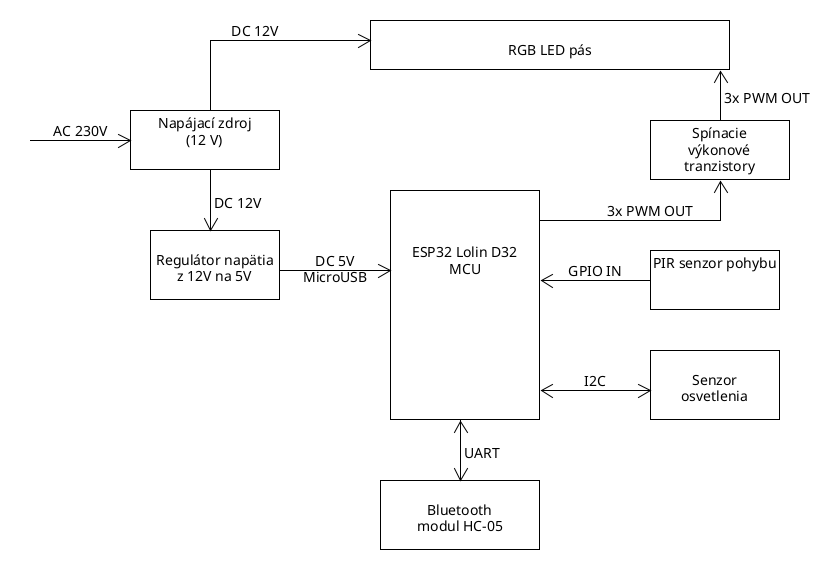
\includegraphics[width=\textwidth]{assets/block-diagram.png}
	\caption{Blokový diagram vnoreného systému inteligentného svietidla}
	\label{fig:block-diagram}
\end{figure}

\begin{figure}[h]
	\centering
	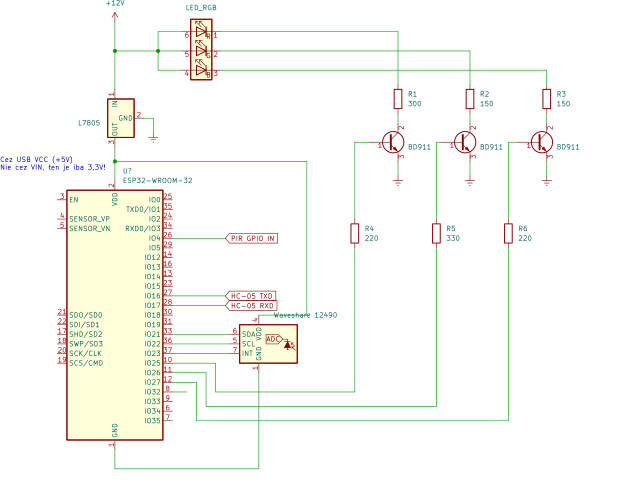
\includegraphics[width=0.8\textwidth]{assets/electrical-schematics.png}
	\caption{Schéma obvodu}
	\label{fig:electrical}
\end{figure}
Na schéme \ref{fig:electrical} je zakreslené zapojenie jednotlivých modulov na piny mikrokontroléra. Piny VCC a GND zo senzorov sú vedené na piny 3,3~V a GND na vývojovej doske ESP32. Bluetooth modul je pripojený priamo na 5~V z L7805. LED pásik už obsahuje rezistory pripojené na kolektory tranzistorov. Bázové rezistory sú zapojené ako prídavné súčiastky.
\FloatBarrier

\subsection{Mobilná aplikácia}
Stav a aktuálne vlastnosti lampy sa budú nastavovať cez rozhranie mobilnej aplikácie  určenú na platformu Android. Wireframe rozloženia tlačidiel a textových polí na vpisovanie čísel sa nachádza na Obr. \ref{fig:app-wireframe}.
\begin{figure}[h]
	\centering
	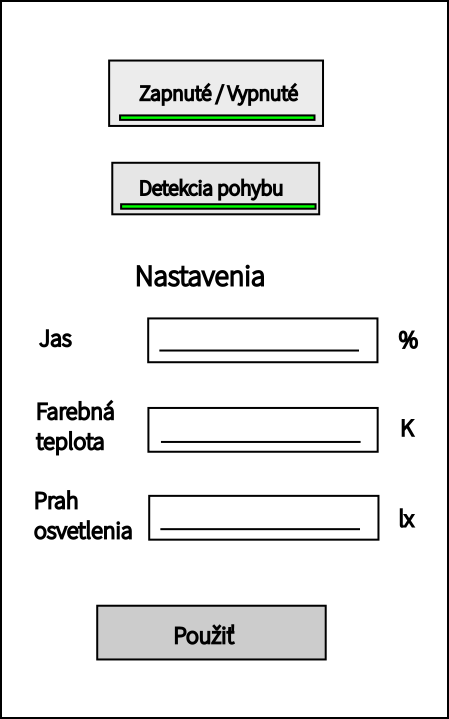
\includegraphics[width=0.28\textwidth]{assets/wireframe.png}
	\caption{Wireframe mobilnej aplikácie}
	\label{fig:app-wireframe}
\end{figure}

Funkcionality aplikácie budú dostupné až po úspešnom naviazaní spojenia s modulom HC-05 cez Bluetooth. Pri pripojení na svietidlo si aplikácia načíta nastavenia uložené na mikrokontroléri do textových polí. Tlačidlo ,,Použiť'' umožní odošlať naraz všetky nastavenia z aplikácie. Na tlačidlách zapnutia svetla a detekcie pohybu, alebo vedľa nich, bude indikovaný aktuálne stav oznamovaný zo zariadenia pri akejkoľvek zmene.
\FloatBarrier

\subsection{Spínanie svetla}
Svetlo sa môže v podstate nachádzať len v dvoch stavoch - zapnuté a vypnuté, aj keď charakter emitovaného svetla môže byť odlišný od situácie. Existuje však viacero scenárov na prepnutie stavu pri návrhu ktorých, je dôležité odstrániť konflikty. Nesmie nastať jav, že sa svetlo rozsvieti aktivovaním jedného pravidla a vzápätí sa zhasne uplatnením iného.
\begin{figure}[h]
    \centering
	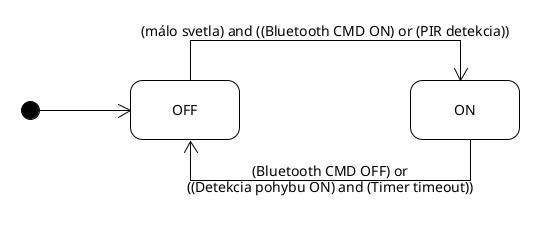
\includegraphics[width=0.7\textwidth]{assets/light-states.png}
	\caption{Stavový diagram spínania svietidla}
	\label{fig:state-diagram-switch}
\end{figure}

\begin{figure}[h]
    \centering
	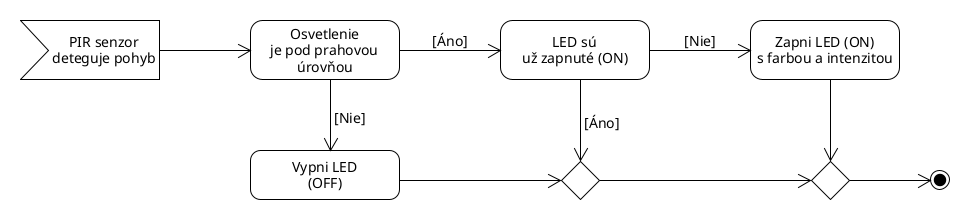
\includegraphics[width=\textwidth]{assets/pir-motion-detect.png}
	\caption{Zapnutie svietidla pri detekcii pohybu}
	\label{fig:pir-motion-detect}
\end{figure}

Pravidlá na prepnutie stavov svetla sú nasledovné (Obr.~\ref{fig:state-diagram-switch}):
\begin{itemize}
\item \textbf{Ak je OFF}: Okolité osvelenie musí byť pod nastavenou prahovou úrovňou: lux~$\leq$~threshold, a súčasne bol poslaný dopyt o zapnutie svetla, buď z mobilnej aplikácie alebo od pohybového senzora.
\item \textbf{Ak je ON}: Mobilná aplikácia poslala dopyt na vypnutie svetla alebo vypršal časovač od posledného dopytu na zapnutie (ten je aktívny vždy keď spustená detekcia pohybu).
\end{itemize}
Postup zapnutia svetla pri detekcii pohybu je ilustrovaný na diagrame (Obr.~\ref{fig:pir-motion-detect}).




%TODO
\section{Opis implementácie}
% Firmvér v ESP-IDF
% Softvér pre Android smartfón
% Formát správ {S/0,M/0,...}

\begin{enumerate}
\item Kelvin ← Temperature
\item Kelvin →RGB (podľa regresného modelu)
\item RGB → HSV
\item V ←brightness
\item HSV→ RGB
\item PWM driver 8-bit OUT
\end{enumerate}



\begin{figure}[h]
\centering
\begin{subfigure}[b]{0.48\textwidth}
	\centering
	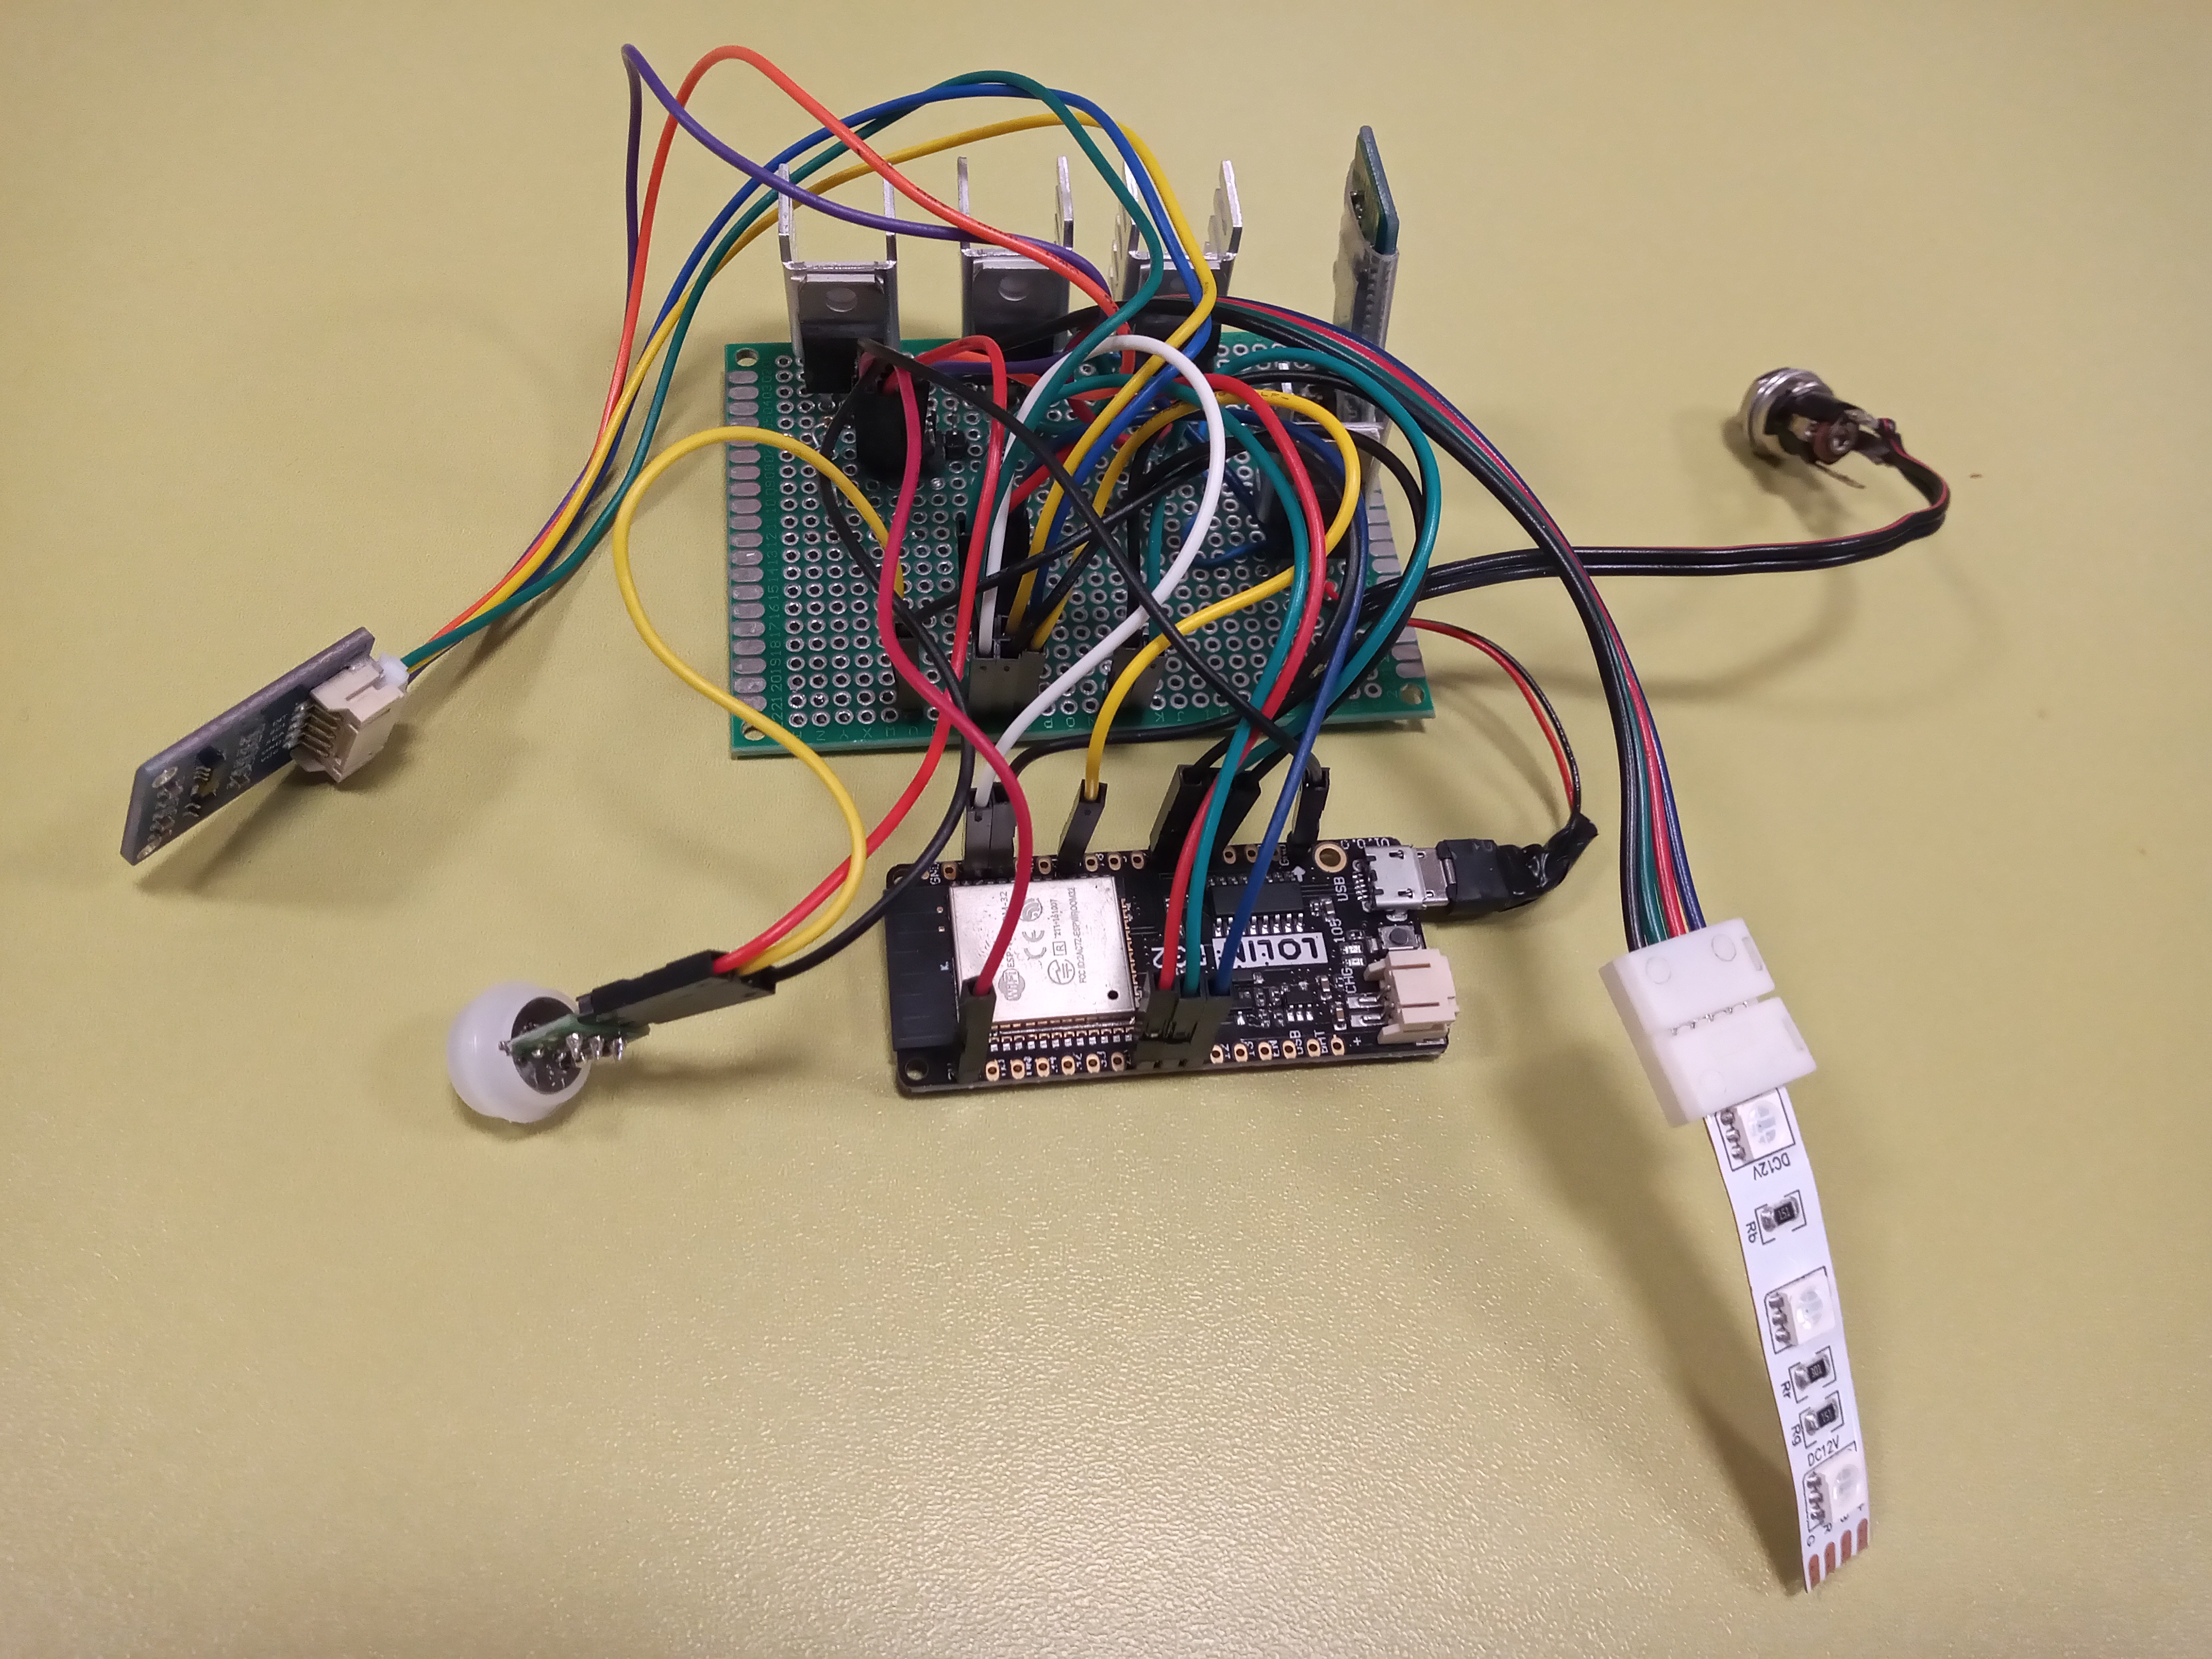
\includegraphics[width=\textwidth]{assets/prototype.jpg}
\end{subfigure}
\hfill
\begin{subfigure}[b]{0.48\textwidth}
	\centering
	\includegraphics[width=\textwidth]{assets/prototype-back.jpg}
\end{subfigure}
\end{figure}

\begin{figure}
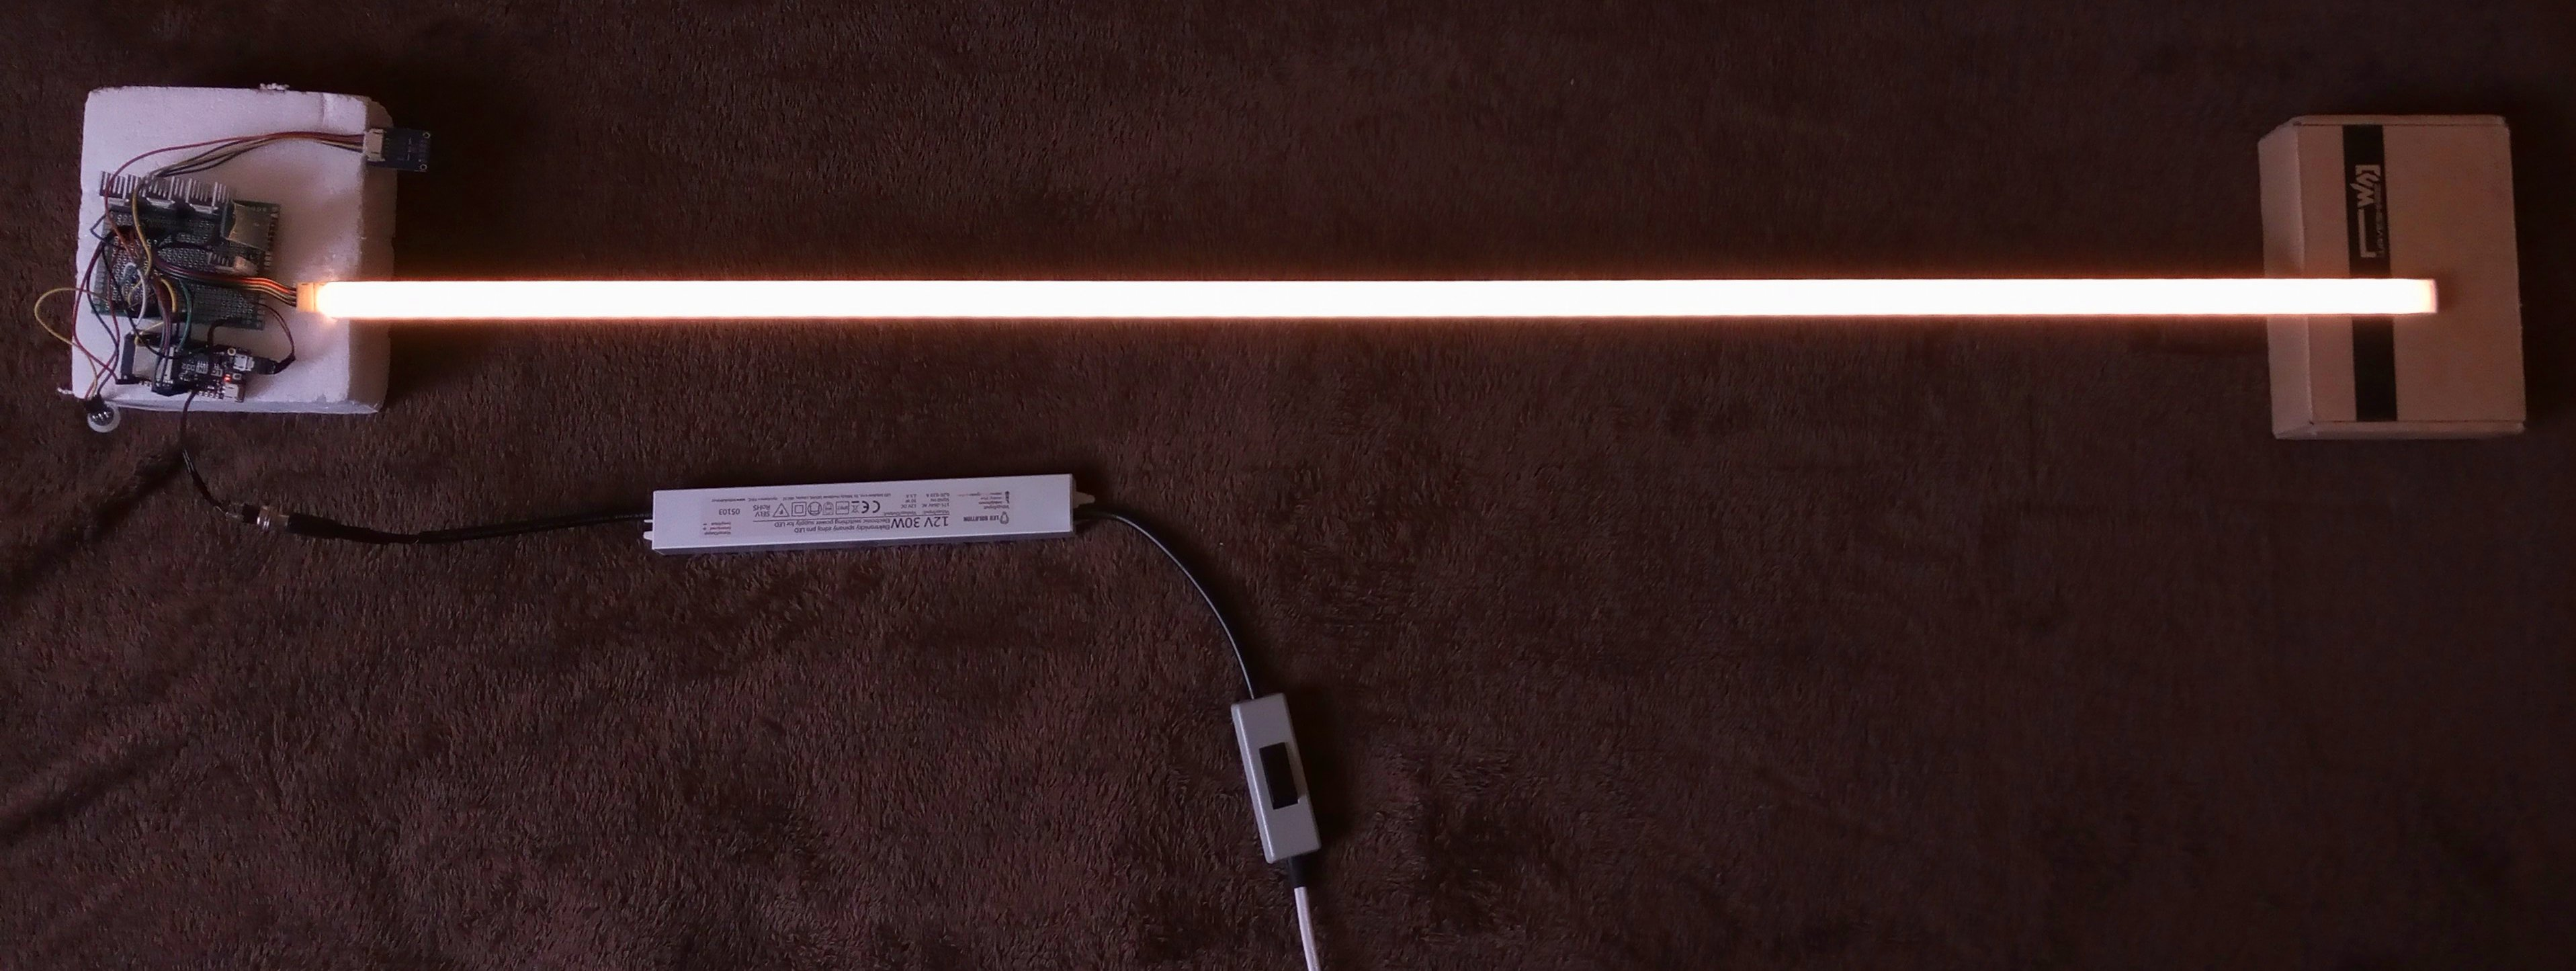
\includegraphics[width=\textwidth]{assets/lamp.jpg}
\end{figure}

\subsection{Nastavenie farby a intenzity svietidla}

\subsection{Firmvér tasky}

% ESP-IDF - C kód a drivers 
% Android studio  (link na dokumentáciu)

\subsection{Mobilná aplikácia}
Obrazovka a popis fungovania

\section{Otestovanie riešenia}
% Testovacie scenáre - Akceptačné testy

% - 

\section{Zhodnotenie výsledkov}

\printbibliography[title={Literatúra}]
\newpage

\section{Technická dokumentácia}
\subsection{Prehľad hardvérových súčiastok}
Na základe predošlej analýzy sme zostavili zoznam súčiastok potrebných pre zhotovenie zariadenia. Cena hardvéru prototypu (jednokusová výroba) je odhadovaná na 55 \texteuro na základe nami zvolených dodávateľov.

\paragraph{Riadiaca jednotka}
\begin{itemize}
\itemsep0pt
\item ESP32 WeMos Lolin D32 - Mikrokontrolér
\item HC-05 - Bluetooth modul
\end{itemize}

\paragraph{Senzory a akčné členy}
\begin{itemize}
\itemsep0pt
\item RGB LED pásik 14,4W/m 12V bez krytia IP20 1m
\item Olimex PIR-SB312 10x8mm 
\item WS-17146 TSL25911 Light Sensor
\end{itemize}

\paragraph{Elektrické súčiastky}
\begin{itemize}
\itemsep0pt
\item L7805CV Lineárny regulátor napätia 12V na 5V
\item NPN Tranzistor BD711 
\item Rezistory - 220 $\Omega$, 330 $\Omega$
\item LED zdroj (trafo) 12V 30W IP67
\item Flexo šnúra – 3m
\item Konektory: RGB LED pásik, Micro USB-B, DC konektor a zásuvka
\end{itemize}

\paragraph{Mechanické súčiastky}
\begin{itemize}
\itemsep0pt
\item DO1 chladič
\item DO3A chladič
\item Univerzálny plošný spoj
\item Nástenný profil N3 biely, Opálový kryt 1m
\item Koncovka profilu N3 biela
\item Vypínač mezišnúrový
\end{itemize}

% Štruktúra priečinkov
% Nahratie firmvéru
% Nahratie softvéru
% FW a SW: Moduly a funkcie

\end{document}